
\chapter{INTRODUCTION} \label{ch:introduction}% Must have a blank line after every section label

\epigraph{\say{Begin at the beginning,} the King said, very gravely, \say{and go on till you come to the end: then stop.}}{Lewis Carroll, \emph{Alice in Wonderland}}

\noindent Humans are a gregarious species. Early in our history, selective pressures favored groups who cooperated for protection and efficient resource allocation. Nowadays, the means by which we interact has evolved. The Internet and telephone networks remove the fetters of physical proximity in forming communities, which can now span broad geographic ranges. Different actions and media for connection define relationships between people, and the aggregation of these people and their links is a social network.

Although numerous fields study human interactions and group behavior---economics, linguistics, political science, and sociology to name a few---network science focuses on the \emph{structure} of these connections, abstracting away the specific nature that defines these connections. This allows the field's methods to be applied to numerous other domains.

An important problem in network science is to detect the communities (sometimes \say{clusters}) present in a network. Grouping the actors based on their interconnections reduces the graph and reveals a \say{mesoscopic} level of complexity~\cite{yang2016comparative}, as well as aiding in the identification of actors' (i.e.\ nodes') roles~\cite{guimera2005functional}. Beyond social network analysis, this problem emerges in taxonomy and phylogeny~\cite{jardine1971mathematical}, analysis of protein function, animal social behavior, traffic planning, and visualization.

As is common, we formulate community detection as an optimization of modularity. Modularity quantifies the separation of a network into distinct, highly interconnected groups. Maximizing modularity is NP-hard.

To solve the optimization problem, we present a polynomial-time approximation method. It greedily maximizes modularity by maximizing max-min fair throughput between all pairs of network nodes. This approximation method is evaluated as a method for determining the mesoscopic, community-level structure. 

\section{Community Structure}

The discipline of community detection rests on the hypothesis that community structure is uniquely encoded in the wiring of the network~\cite{barabasi2016network}. The relationships between actors alone specify the communities, without the need for external information. For this reason, the \emph{graph} is an abstract data type for representing a network that is central to the study of network science and community structure. In literature, the terms \emph{network} and \emph{graph} are interchangeable. Networks generally consist of \emph{nodes} with \emph{links} between them, while the corresponding terms for graphs are typically \emph{vertices} and \emph{edges}. In this thesis, we use the terminology \emph{nodes} and \emph{edges}.

Random graphs have no structure~\cite{barabasi2016network}. The distribution of their edges is statistically homogeneous, and the degrees of nodes are similar~\cite{erdos1959random}. By contrast, the edge distribution tends to clump in real world networks~\cite{fortunato2010community}. This creates regions of high and low interconnectivity. These differences in connection motivate the concept of a \emph{community}. (See \autoref{fig:florentine_dendrogram}.)

\begin{figure}
	\centering
	\begin{minipage}{0.525\linewidth}
		\centering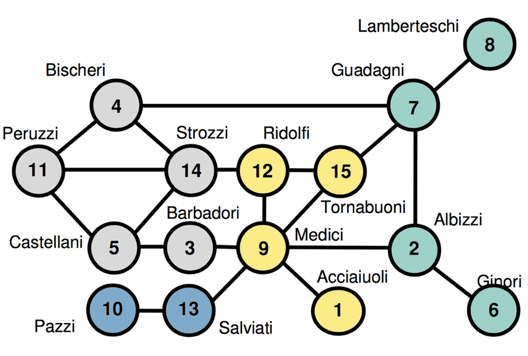
\includegraphics[width=\linewidth]{fig/florentine_cluster}
	\end{minipage}
	\begin{minipage}{0.375\linewidth}
		\centering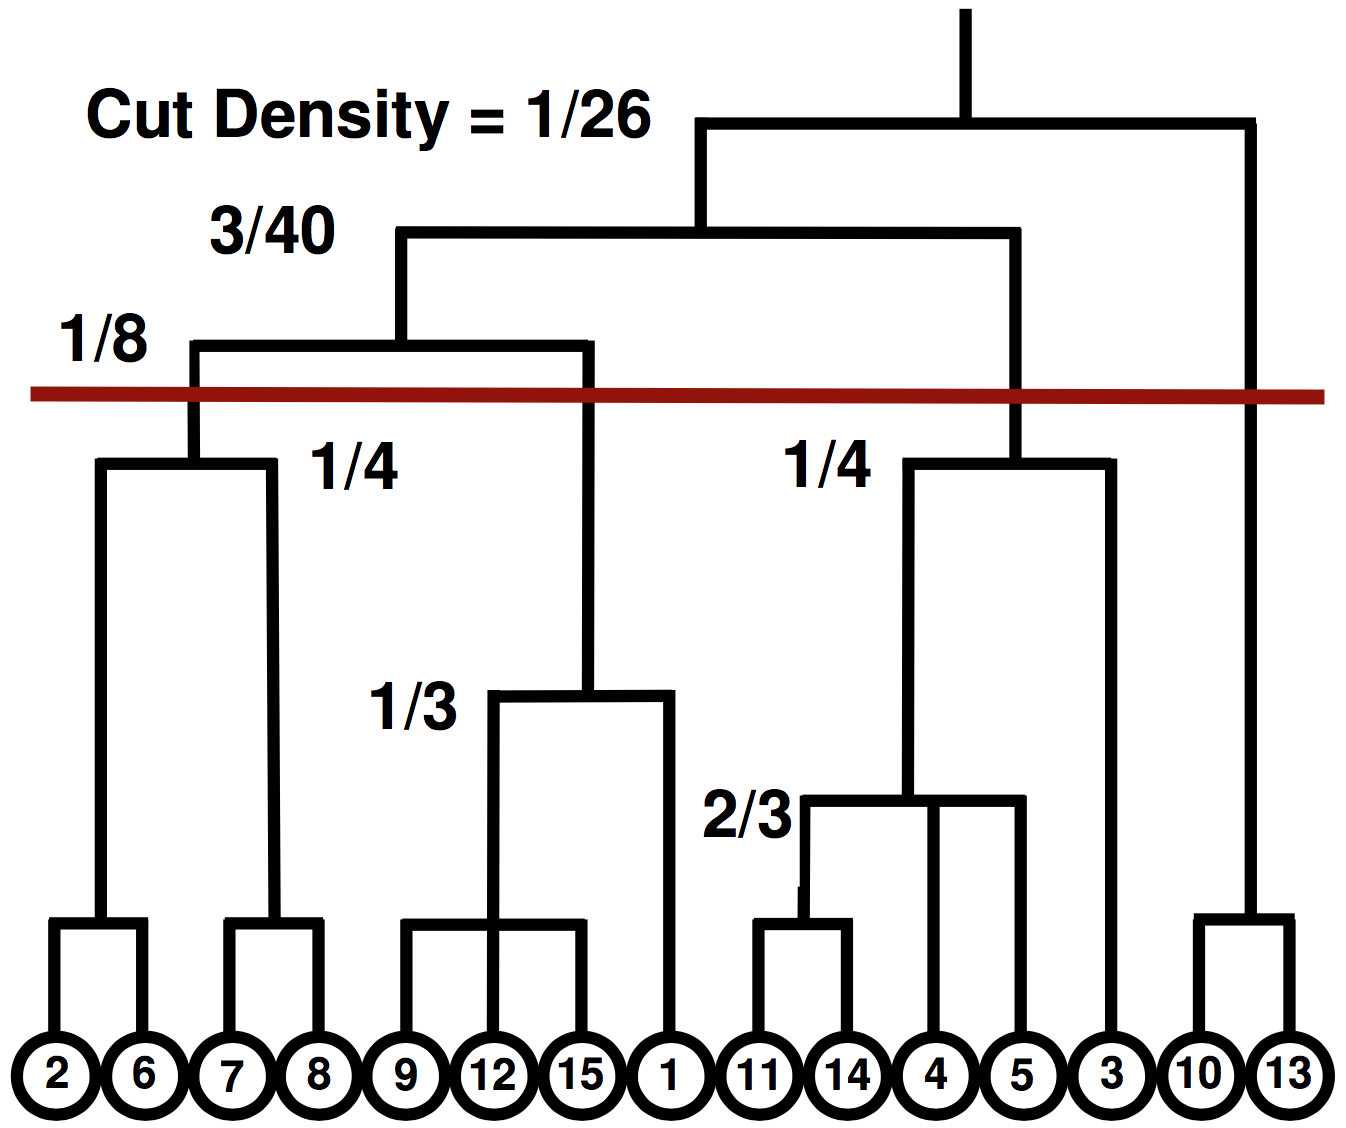
\includegraphics[width=\linewidth]{fig/florentine_dendrogram}
	\end{minipage}
	\caption{\textbf{(a)}~Padgett's Florentine families network~\cite{padgett1993robust}, in clusters (communities) of maximum modularity as determined by the MCF cut algorithm~\cite{mann2008sparsest}. Note the high intra-community linkage and low inter-community linkage. \textbf{(b)}~The dendrogram of the Florentine families network as determined by the MCF cut algorithm. The vertical axis represents the cut density of each split, a measure of similarity between clusters. The red line indicates the level of the flat clustering with maximum modularity: the four communities shown in~\textbf{(a)}.}
	\label{fig:florentine_dendrogram}
\end{figure}


There is no consensus on the definition of a community~\cite{hu2008comparative}, which may contribute to the multitude of methods which identify them: Each is well-suited for its own notion. Radicchi et al.\ provide a pair of potential definitions based on node degree~\cite{radicchi2004defining}:
\begin{definition}Strong community

\emph{Each} node in the community has more intra-community than inter-community connections.\end{definition}

\begin{definition}Weak community

The \emph{average} intra-community degree exceeds the \emph{average} inter-community degree.
\end{definition}
Mann claims that edge density, the fraction of edges present relative to the number of potential edges, gives a clearer definition of density~\cite{mann2008extensions}:
\begin{definition}Density-based community

A subgraph with high edge density, with low edge density between it and the rest of the graph.

\end{definition}
Our discussion will rely on each of these three definitions.



\subsection{Hierarchical Communities}

A community may have sub-communities which are even tighter-knit within itself. This nested structure forms a hierarchy. Hierarchical structure can be used to identify functional relationships within and between clusters and predict missing links in the network~\cite{clauset2008hierarchical}. The cluster hierarchy is commonly presented as a dendrogram (e.g. \autoref{fig:florentine_dendrogram}), with some metric of similarity or distance (i.e. dissimilarity) along the vertical axis.

Methods for determining hierarchical communities fall under two general regimes~\cite{sneath1962numerical}:

\begin{description}

\item[Divisive (i.e. top-down) methods.] Starting from all nodes in one community, these methods recursively split the graph into sub-communities, working their way down. Once separated, clusters are never re-joined. An exhaustive search is $O(2^n)$, so popular methods are not exhaustive. 

\item[Agglomerative (i.e.\ bottom-up) methods.] Nodes begin as singletons that are merged into communities recursively. Once joined, clusters are never separated, so these methods are sensitive to early decisions. The methods, in general, have a computational complexity in $O(n^2 \log(n))$~\cite{rokach2005clustering}, though some $O(n^2)$ methods have been proposed~\cite{defays1977efficient, sibson1973slink, day1984efficient}.

\end{description}

We are in need of a conceptual framework for the hierarchical clustering process. Campello et al.~\cite{campello2013density} identify five steps to the process of hierarchical clustering on points in a metric space (as opposed to graphs):

\begin{enumerate}
\item Transform the space according to the density/sparsity.
\item Build the minimum spanning tree (MST) of the distance weighted graph.
\item Construct a cluster hierarchy of connected components.
\item Condense the cluster hierarchy based on minimum cluster size.
\item Extract the stable clusters from the condensed tree.
\end{enumerate}

Methods have long been known for embedding graphs into metric spaces for clustering and multi-commodity flows so that this process can been used. However, they introduce a systematic bias~\cite{linial1995geometry}. Further, a single graph can have multiple MSTs, so the choice of one is arbitrary. This leads to inconsistent results. To eliminate these sources of discrepancy, I will ignore points in metric space and focus only on clustering un-embedded graphs. The final three steps are the essential ones employed by hierarchical community detection algorithms.



\subsection{Flat Cluster Extraction} \label{sec:flat cluster extraction}

While nested communities may be relevant for certain applications, many use-cases seek a flat clustering of the nodes in a graph from a hierarchical clustering method. A flat clustering is a partitional assignment of every node to a single community, as opposed to an assignment into overlapping or nested communities\footnote{Jardine and Sibson provide an unrelated definition of a \say{flat cluster method}~\cite{jardine1971mathematical}. In this paper, I use Campello et al.'s definition of \say{flat clustering}~\cite{campello2013framework}.}~\cite{campello2013framework}. Hierarchical clustering methods present a variety of potential flat clusterings, from which one must be chosen.

Informally, flat cluster extraction is often done by drawing a horizontal line across the dendrogram at some height: select the clusters crossed by the line. Non-hierarchical algorithms sidestep this process to deliver flat clusters.

\emph{Modularity} maximization (described in \autoref{sec:modularity}) is the de facto standard for determining the optimal group of communities. It measures the tendency for groups to have dense connectivity within and weak connectivity without, codifying intuition about the meaning of a community. 
%Mann experimented with this as well as maximization of the clustering coefficient. 
Another method adaptively selects clusters with maximum stability across the entire dendrogram, rather than cutting across a particular level~\cite{campello2013density}. When every node \emph{must} be assigned to a cluster, the stability idea is largely similar.



\section{Modularity} \label{sec:modularity}

Lacking a definition of \say{communities} makes it hard to reconstruct the existing communities in a graph. Further, when ground truth communities are not known, we need a measure to judge the quality of communities. The common practice is to maximize modularity~$Q$, a measurement of the quality of a clustering~$\mathcal{C} = \{C_1, \ldots, C_t\}$~\cite{newman2006modularity}. Brandes et al.~\cite{brandes2007finding}
present the formula as:
\begin{equation}
Q (\mathcal{C}) = \sum_{C \in \mathcal{C}} \left( \frac{| E(C) |}{m} -  \left( \frac{\sum_{v \in C} \deg(v)}{2m} \right) ^2 \right)
\label{eqn: modularity}
\end{equation}
Here, $m$~represents the number of edges, and $E(C)$~represents the edges internal to cluster~$C$. Modularity balances the objectives of many edges within clusters (the first term) and avoiding giant, all-encompassing communities (the second term). Highest scores are achieved by eliminating edges in sparse regions of the graph, which reflects intuition about communities. The value of~$Q$ can range from $-1/2$ (when the graph is partitioned into singletons, so no edges are contained) to $1$ (in the special case that no edges \emph{exist}, so $|E(C)|$ is defined as $1$.)~\cite{brandes2007finding}.

Another way to frame modularity is a comparison of the arrangement of edges against a random null model: one where every node maintains the same degree, but edges are randomly connected between them. Imagine that every node has the same number of half-edges, or \emph{stubs}, as its degree. These stubs can be connected together in any way. Modularity compares the number of edges within communities to the expected number according to this random null model. More edges than expected within each community gives a higher score.

All metrics of clustering quality have a limit to their ability to perceive communities~\cite{fortunato2007resolution}. Modularity's resolution limit comes from the configuration model just described, which assumes an equal likelihood of any two stubs being attached. As the network size grows, the expected number of edges between two communities approaches zero, so an extant edge between the communities is treated by modularity optimization methods as a sign that the communities should be joined (for bottom-up methods) or not separated (for top down methods). Further, in large real-world networks, the assumption that \emph{any} two edges can be joined is unrealistic: A node's sphere of influence will generally be a small part of the network~\cite{fortunato2007resolution, good2010performance}. Despite the resolution limit, modularity remains the preferred metric for evaluating clusterings. Small and medium networks are used in the remainder of this work, so the resolution limit is not approached.

Maximizing modularity directly is NP-hard~\cite{brandes2006maximizing}; it can be done using integer linear programming (ILP)~\cite{brandes2007finding}. This motivates approximations. 



\section{Approximation}

To approximate optimal modularity, we create another optimization problem: 
producing the \emph{sparsest cuts} of the graph. A sparsest cut is a set of edges of minimal density: Compared to the number of \emph{possible} edges between groups separated by the sparsest cut, the number of \emph{existing} edges is minimal. 

As identifying sparsest cuts is also NP-hard~\cite{matula1990sparsest}, we approximate their identification by a heuristic. This is the weak dual problem to the sparsest cut problem: producing \emph{max-min fair flow} (defined below) between all pairs of nodes. Although the method was first described by Matula in 1983~\cite{matula1983cluster}, the increase in computing power over the last three decades makes it possible to apply the method to networks of nontrivial size. We are able to assess its practicality on real-world problems.

Max-min fairness means that increasing the flow between a pair can only be achieved by decreasing the allocation to a pair with equal or less allocation~\cite{le2005rate}. In other words, no one's standing can be improved except by taking from those who are as well off or worse off. The method for finding this fair allocation successively divides the graph into hierarchical communities.

The method begins by maximizing the level of allocation between all pairs, which will saturate a set of edges (the \emph{cut set}) with flow. (This maximization problem is called the maximum concurrent flow problem, or MCFP.) These edges separate the graph into two or more components, forming the first level of the dendrogram. Flow between certain pairs cannot be maximized further; it is constrained by the capacity of the cut. The allocation between these pairs is then fixed, and we iteratively maximize the next amount of flow, and the next, until all flows are fixed and the entire graph is saturated. The level of allocation, or \emph{throughput}, for each cut orders the separation of hierarchical clusters in the dendrogram. 

The maximization at each level is done using a \emph{linear program}. An introduction to relevant linear programming (a.k.a.\ linear optimization) concepts is given in \autoref{app:LP}. The structure of the relevant linear program is given in \autoref{ch:algorithm}. Finally, to extract flat clusters, we cut the dendrogram at the level with maximal modularity.

Solving linear programs (LPs) and computing modularity are both possible in polynomial time. This means that finding a clustering with maximal modularity using this method is asymptotically faster than finding the maximum possible modularity, which is an NP-hard problem.

%Mann~\cite{mann2008sparsest} presented a community detection algorithm, the \emph{maximum concurrent flow (MCF) cut algorithm}, that identifies the hierarchical structure of a network. It treats the network as a flow network, iteratively finding constraining cuts\todo{What were these called?} by solving the maximum concurrent flow problem~\cite{matula1985concurrent}. The MCF cut algorithm computes a \emph{divisive average linkage}, trading the runtime of Sokal and Michener's agglomerative average linkage~\cite{sokal1958statistical} for robustness toward initial conditions. (Agglomerative methods cannot backtrack their decisions, making them extremely sensitive to early decisions.) The MCF cut algorithm outperformed the popular Girvan--Newman algorithm~\cite{girvan2002community} on small real-world networks and a popular synthetic benchmark. In addition, the MCF cut algorithm gave rise to a canonical measure of node centrality called \say{flowthrough centrality}.
%
%% \subsection{The importance of exploring this thing}
%
%At the same time, a number of other community detection algorithms emerged~\cite{clauset2004finding, rosvall2007information, rosvall2009map, raghavan2007near, newman2006finding, blondel2008fast, reichardt2006statistical, pons2005computing, pares2017fluid}. Since the MCF cut and maximin algorithms were presented, new benchmarks for assessing the quality of community detection have been proposed, better matching properties of real-world networks~\cite{lancichinetti2008benchmark}. It is important to assess the MCF cut and maximin algorithms in these contexts to better understand their relevance and weaknesses.

%Mann's method builds on the maximum concurrent flow problem (MCFP), first investigated by Matula~\cite{matula1985concurrent}. Mann presents the \emph{hierarchical} MCFP as the basis for clustering. The method identifies a set of saturated edges as the basis of a a $k$-partite cut. Next, it fixes the current demand between all pairs and selects the largest component to continue solving. Relevant parts of the algorithm are expanded upon in the remaining chapters as they emerge.
%
%This investigation focuses on an evolution of Mann's MCF cut algorithm. Mann used this algorithm, first presented by Matula~\cite{matula1983cluster}, to compute a canonical centrality measure for graphs; however, he did not apply it to the problem of community detection. The improvement is a maximin algorithm that keeps the entire network in play as it increases flow~\cite{matula1983cluster}, rather than processing the induced components independently of one another. This provides greater robustness toward changes in edge weights and can identify \emph{repeated} cuts on already-saturated edges. The significance of these cuts is discussed in \autoref{ch:robustness}.
%
%The maximin algorithm is so named because it works to maximize the minimum throughput between every pair. 

\section{Structure of the Remaining Chapters}

A survey of popular community detection techniques is presented in \autoref{ch:literature}. The chapter also spans advances in the problem of max-min fair flow allocation, especially as they pertain to the problem of community detection.

\autoref{ch:algorithm} gives the leximin method for community detection and provides an outline of its properties. It additionally contrasts it with the related MCF cut method of Matula and Mann~\cite{mann2008extensions, matula1985concurrent}.

In \autoref{ch:robustness}, I show that the leximin method is more robust toward perturbations in the graph than competing methods. Further, I show that, unlike popular methods, it is capable of showing ties in cuts. I explain why finding ties is desirable.

The leximin method possesses an unusual property, which is an extension of its ability to reveal ties. When a graph (or subgraph) is sufficiently unstructured the leximin algorithm will not attempt to partition the graph (or subgraph). In these cases, flow simultaneously saturates all edges in a community or communities, fragmenting the community into singletons. I refer to this saturation as \emph{gridlock}, and I explore it in \autoref{ch:random}. I show that for every graph that exhibits gridlock, there exists an unweighted multigraph with the same concurrent flow assigned to edge-disjoint paths between all pairs.

In \autoref{ch:comparison}, I compare the leximin method against common methods identified in \autoref{ch:literature} on a standard benchmark and show that it performs with similar accuracy to existing methods. I explain that for networks with weak communities, gridlock is frequent. The common metric for appraising community detection quality, normalized mutual information, inflates the score of a graph that gridlocks. I use this to argue in favor of a related, existing metric that adjusts for this: adjusted mutual information.

Finally, in \autoref{ch:conclusion}, I conclude and describe future directions.

%
% \subsection{Talk about its ``competitive advantage''}
%
%The properties of the maximin and MCF cut algorithms are explored in \autoref{ch:robustness}. Particularly, the robustness toward variation in edge weight is demonstrated, showing an improvement over popular hierarchical algorithms. \todo{Results.}
%
% \subsection{Comparison}
%
%The MCF cut algorithm was developed at a turning point in the field of network science; afterward, more refined tools emerged. \todo{How do I talk about the minimax algorithm fitting in?}I compare the MCF cut algorithm against \emph{modern} community detection algorithms on a \emph{modern} benchmark in \autoref{ch:comparison}. This is important for contextualizing the MCF cut algorithm. \todo{Results.}
%
%
% \subsection{Introduce that other thing: role-labeling}
%
%An extension of the HMCFP (and thereby, the MCF cut and maximin algorithms) to directed, weighted graphs is presented in \autoref{ch:directed}.
%
%

%\section{Characterizing network roles}
%
%\url{https://arxiv.org/pdf/cond-mat/0505185.pdf}
%
%- vulnerability
%
%- rich club coefficient
%
%- degree distribution
%
%\hrule
%
